\subsection{Image Morphology}

Some image processing pipelines stand to benefit from structured data processing \cite{donenfeld_unified_2022}.
%
We focus on binary image morpology and the logical transformation of binary images and masks.
%
We consider two operations: binary erosion (computing a mask), and a masked histogram (using a mask to avoid work).
%
We use images are all binary, either by design or having been thresholded.

Finch allows us choose our datastructure, so we may choose to use either a dense representation with bytes ($Dense(Element(0x00))$), a bit-packed representation ($Dense(Element(UInt64))$), or a run-length encoded representation that represents runs of true or false ($SparseRLE(Pattern())$).
%
All of these have their advantages.
%
The dense representation induces the least overhead, the bit-packed representation can take advantage of bitwise binary ops, and the run-length encoded version only uses memory and compute when the pattern changes. % between true and false.

Similarly, since Finch let's us choose our algorithm we can implement erosion in a few ways.
%
The erosion operation turns off a pixel unless all of it's neighbors are on.
%
This can be used to shrink the boundaries of a mask, and remove point instances of noise \cite{fisher_hypermedia_1996}.
%\help{link a few cool images that show erosion}
%
This introduces three instances of structure in the control flow: the mask, the padding of inputs, and the convolutional filter.
%
We focused on the filter.
%Note that three instances of structured data are used here, both in the mask, in the padding of the inputs, and in the convolutional filter itself.
%
We might understand the filter as a structured tensor of circular shifts, or we might understand each shifted view of the data in an unrolled stencil computation as a structured tensor, or a two part stencil where we compute the horizontal then vertical part of the stencil.
%
We experimented with these options and found that the last approach performed best, due to fitting the storage formats while reducing the amount of work with intermediate temporaries.
%
Figure \ref{fig:morphology_listing} displays example erosion algorithms for bitwise
or run-length-encoded algorithms.
%
% and a masked histogram kernel.

We compared against OpenCV.
%
We used four datasets. We randomly selected 100 images from the MNIST \cite{lecun_gradient-based_1998} and Omniglot \cite{lake_human-level_2015} character recognition datasets, as well as a dataset of human line drawings \cite{eitz_how_2012}. 
%
We also hand-selected a subset of mask images (these images were less homogenous, so we listed them in Appendix C) from a digital image processing textbook \cite{gonzalez_digital_2006}. 
%
All images were thresholded, and we also include versions of the images that have been magnified before thresholding, to induce larger constant regions. 
%
IN our erosion task, the sparseRLE format performs the best as it is asymptotically faster and uses less memory, leading to a 19.5X speedup over OpenCV on the sketches dataset, which becomes arbitrarily large as we magnify the images (here shown as 266X). 
%
We believe the 51.6x on MNIST is due to calling overhead in OpenCV). 
%
The bitwise kernels were effective as well, and would be more effective on datasets with less structure. 
%
A strength of Finch is that it supports structured datasets, even over bitwise operations, allowing us to implement the bitwise kernel and then mask it.

We also implemented a histogram kernel.
%
We used an indirect access into the output to implement this (Figure \ref{fig:morphology_listing}), something not many sparse frameworks support.
%
We compare to OpenCV since the OpenCV histogram function also accepts a mask. 
%
If we use $SparseRLE(Pattern())$ for our mask, we can reduce the branching
in the masked kernel and get better performance.
%
The improvements with SparseRLE are seen in the histogram task too, as it allows us to mask off contiguous regions of computation, instead of individual pixels, reducing the branches and leading to a significant speedup (20.3x on Omniglot and 20.8x on sketches).
%
%
%A strength of Finch is that it supports structured datasets, even over bitwise operations, allowing us to implement the bitwise kernel and then mask it.

\begin{figure}
    \scriptsize
    \begin{minipage}{0.5\linewidth}
    Wordwise Erosion:
    \begin{minted}{julia}
        output .= false
        for y = _
          tmp .= false
          for x = _
            tmp[x] = coalesce(input[x, ~(y-1)], true) & input[x, y] & coalesce(input[x, ~(y+1)], true)
          end
          for x = _
            output[x, y] = coalesce(tmp[~(x-1)], true) & tmp[x] & coalesce(tmp[~(x+1)], true)
          end
        end
    \end{minted}
    \vspace{12pt}
    Masked Histogram:
    \begin{minted}{julia}
        bins .= 0 
        for x=_
          for y=_
            if mask[y, x]
              bins[div(img[y, x], 16) + 1] += 1
            end
          end
        end
    \end{minted}
    \end{minipage}%
    \begin{minipage}{0.5\linewidth}
    Bitwise Erosion:
    \begin{minted}{julia}
        output .= 0
        for y = _
          tmp .= 0
          for x = _
            if mask[x, y]
              tmp[x] = coalesce(input[x, ~(y-1)], 0xFFFFFFFF) & input[x, y] & coalesce(input[x, ~(y+1)], 0xFFFFFFFF)
            end
          end
          for x = _
            if mask[x, y]
              let tl = coalesce(tmp[~(x-1)], 0xFFFFFFFF), t = tmp[x], tr = coalesce(tmp[~(x+1)], 0xFFFFFFFF)
                let res = ((tr << (8 * sizeof(UInt) - 1)) | (t >> 1)) & t & ((t << 1) | (tl >> (8 * sizeof(UInt) - 1)))
                  output[x, y] = res
                end
              end
            end
          end
        end
    \end{minted}
    \end{minipage}
    \vspace{-12pt}
    \caption{Two approaches to erosion in Finch. The $coalesce$ function defines the out of bounds value. On left, the naive approach. On $SparseRLE(Pattern())$ inputs, this only performs operations at the boundaries of constant regions. On right, a bitwise approach, using a mask to limit work to nonzero blocks of bits.}
    \label{fig:morphology_listing}
\end{figure}

\begin{figure}
	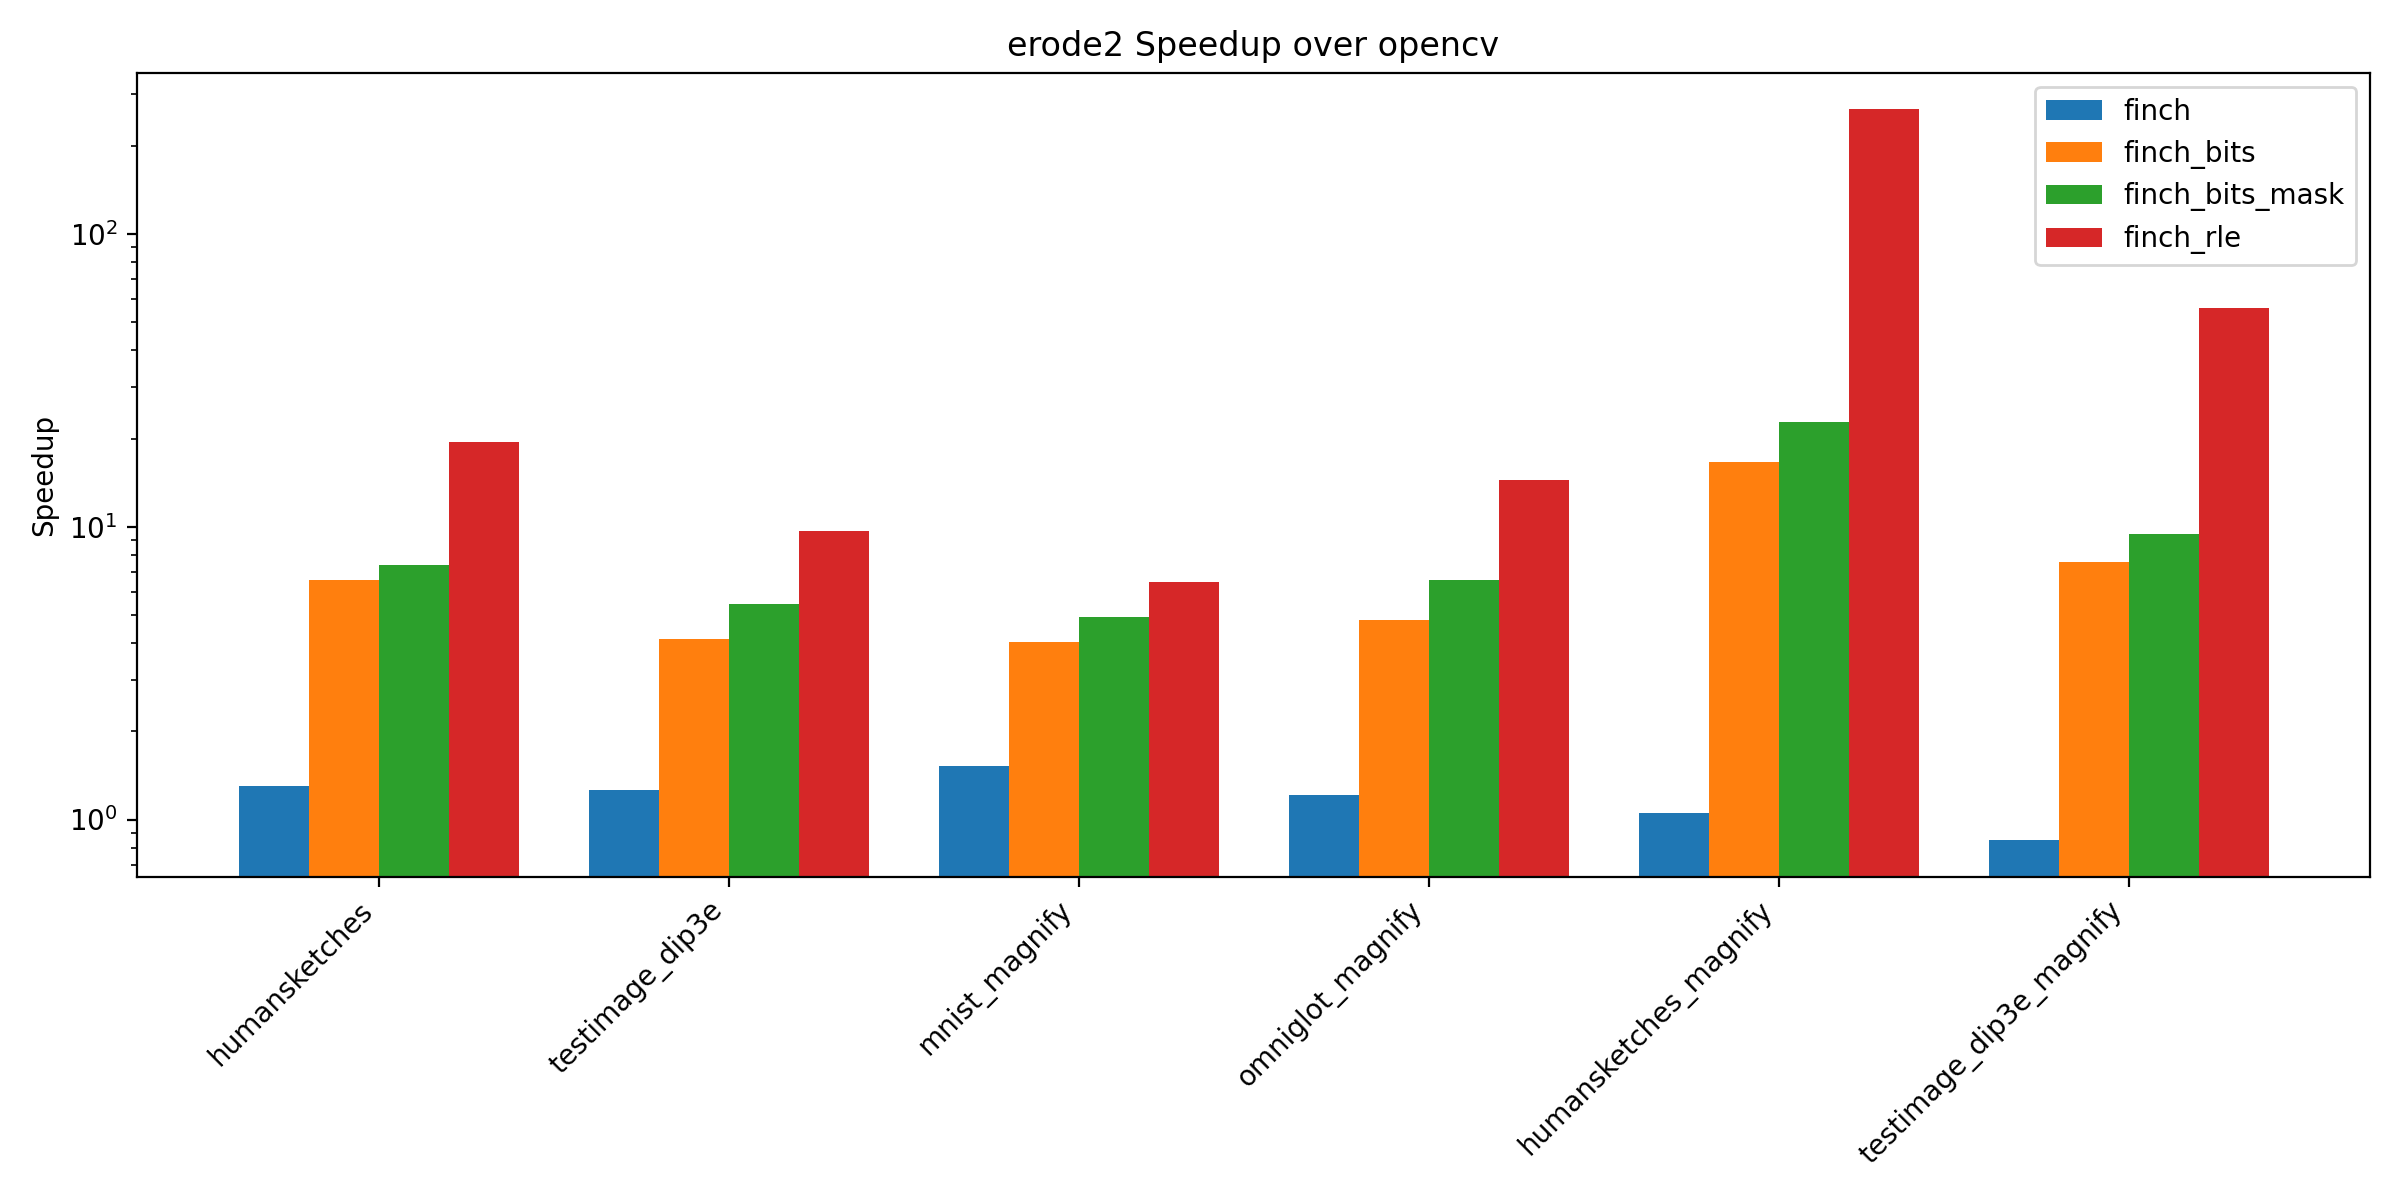
\includegraphics[width=0.5\linewidth]{erode2_speedup_over_opencv.png}%
	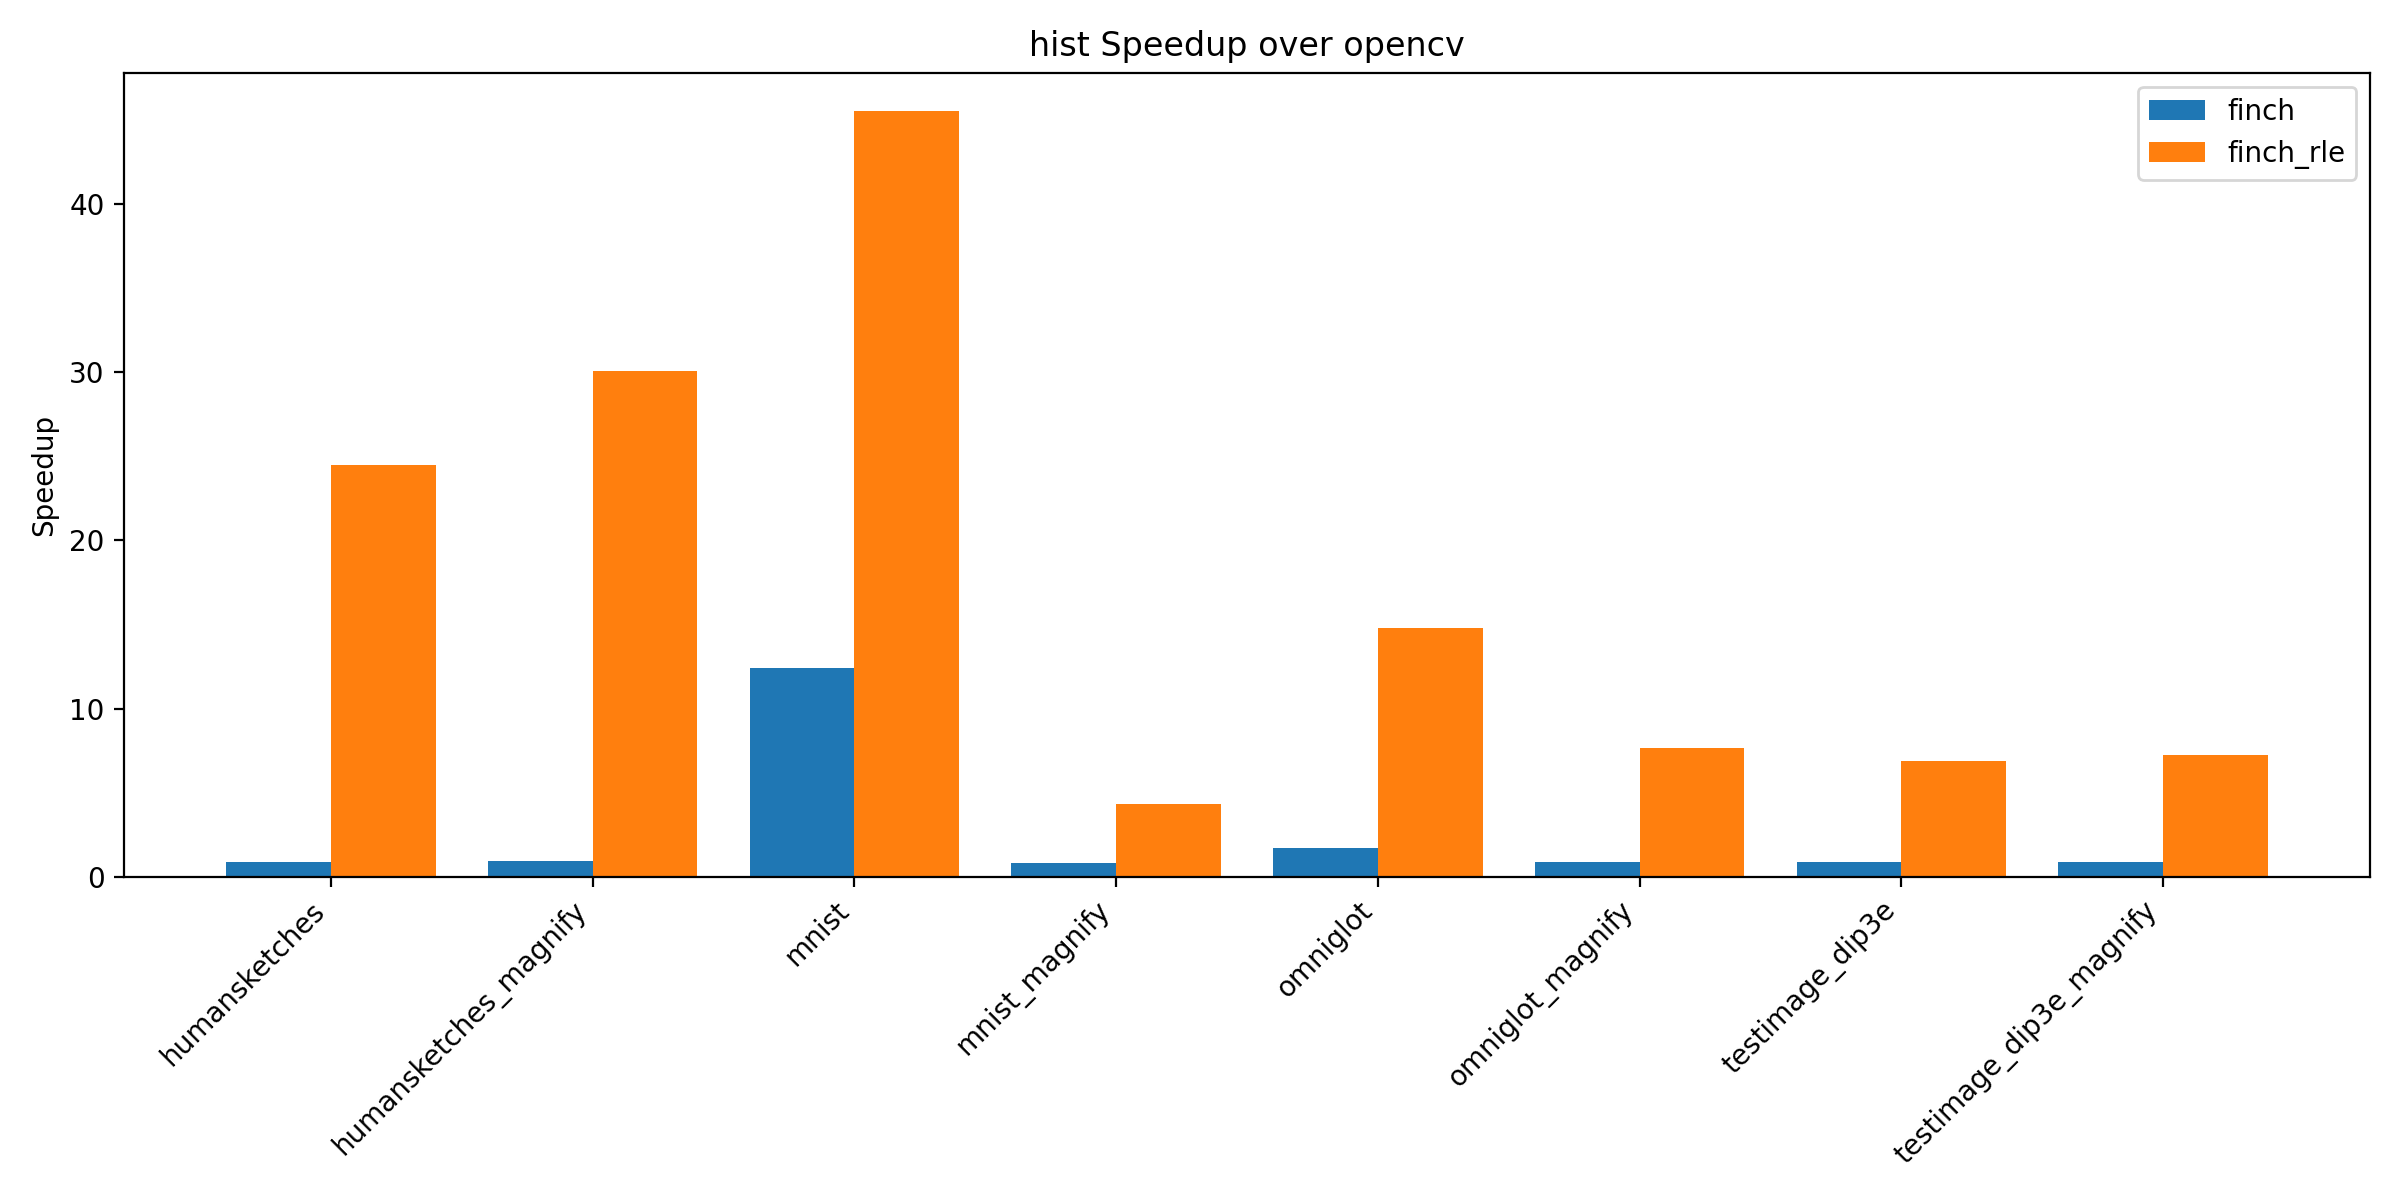
\includegraphics[width=0.5\linewidth]{hist_speedup_over_opencv.png}
 \vspace{-12pt}
    \caption{Performance of Finch on image morphology tasks. On left, we run 2 iterations of erosion. On right, we run a masked histogram.}\label{fig:morphology}
\end{figure}